\chapter{Detailed design}

\section{Actor model}



\section{Rooms}

\subsection{ServerRoom}
\begin{figure}[H]
	\centering
	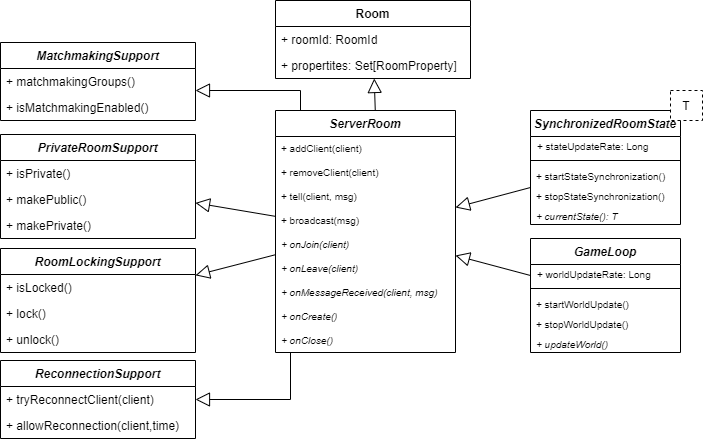
\includegraphics[scale=0.5]{images/4-design/server-room.png}
	\caption{Server room class diagram}
	\label{fig:server_room_class_diagram}
\end{figure}
\texttt{ServerRoom} is a trait that encapsulate the concept of room used server-side; as we see in figure \ref{fig:server_room_class_diagram} it extends the \texttt{Room} trait adding methods to manage clients (add,remove, tell and broadcast) and defining abstract handlers for room events. These handlers are the ones that the developer must implement to define his own type of rooms.

Since the developer may also want to automatically synchronize the state of the game and have an inner game loop (requirements 2.1.2.1 and 2.1.2.2), there are two extension of the server room: \texttt{SynchronizedRoomState} and \texttt{GameLoop} that provide this functionalities. 

The first one is a trait generic in the type of the state that needs to be synchronized to clients; this trait has all methods implemented except for \texttt{currentState} that must be defined by the user and will be called periodically at the specified rate: \texttt{stateUpdateRate}.

The second one, \texttt{Gameloop}, is also a trait but is not generic and requires to define \texttt{updateWorld}, a void method that will be called every \texttt{worldUpdateRate} milliseconds.

While this two traits can be optionally mixed in a ServerRoom, all those that in figure \ref{fig:server_room_class_diagram} are shown on the left, are functionalities that a room has by default:
\begin{itemize}
	\item \texttt{MatchmakingSupport}: gives the developer access to the matchmaking groups that the matchmaking service associated with this room has created.
	\item \texttt{ProvateRoomSupport}: used to set a password to the room in order to prevent access to some clients.
	\item \texttt{RoomLockingSupport}: enables lock and unlock functionalities to the room. 
	\item \texttt{ReconnectionSupport}: allows clients to reconnect to the room within a certain period of time.
\end{itemize}

\subsection{ClientRoom}

\subsection{Properties and Filters}


\section{Server}
Class diagram in figure \ref{fig:server_class_diagram} describes in detail the server architecture displaying the main functionalities of the classes and showing how actors interact with all the other components. 
\begin{figure}[h]
	\hspace*{-1.1in}
	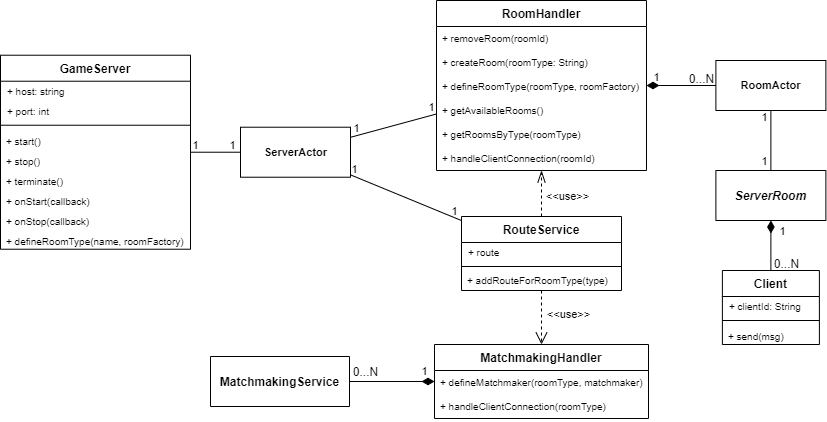
\includegraphics[scale=0.55]{images/4-design/server_class.png}
	\caption{Server class diagram}
	\label{fig:server_class_diagram}
\end{figure}

The \texttt{GameServer} class is the facade interface that is exposed to the developer. It internally creates a \texttt{ServerActor} that is the entity that acts as the real server listening for clients requests. This actor creates a \texttt{RouteService} object that is used to know which routes to use and how to handle requests; it also allows to dynamically define new room types that will be used by te server. 

The \texttt{ServerActor} also uses a \texttt{RoomHandler} to create and define rooms from the server. The same RoomHandler used by the RouteService.

As we described for the server architecture in section \ref{sec:server_arch}, the purpose of the \texttt{RoomHandler} is to manage the active rooms in the applications. Specifically though it doesn't directly create rooms but instead it creates \texttt{RoomActors}: actors used as 'wrappers' for ServerRooms to avoid concurrency issues; more than one client can indeed interact with a single room at the same time, so, in order to avoid race coditions, we decided to make clients communicate with RoomActors that process messages sequentially. Each actor is in charge of notifying clients' actions to the room that is associated with.

Each \texttt{ServerRoom} is linked to an actor and keeps track of connected clients (\texttt{Client} class in figure). Clients are uniquely identified by their id and expose a \texttt{send} method that allows to send messages to them. It is important to notice that each room has its own view of clients: the same client connected to different rooms will have a different id in each of them. 

Clients are also used by the \texttt{MatchmakingService} since is the actor that performs matchmaking operations and needs to know which clients are waiting to start a match. \texttt{MatchmakingService} actors are spawned during server startup if the developer used the \texttt{defineRoomWithMatchmaking} method to define a room. 

Since clients can make requests for matchmaking, the \texttt{RouteService} use a \texttt{MatchmakingHandler} to redirect those requests to the right \texttt{MatchmakingService} actor.


\section{Client}

\section{Communication}\label{sec:communication_design}


\subsection{Json Serialization}
For Request-Response interaction (described in section 3.4), we decided to use json format for both client requests and server responses. We have defined a class that provides json-formatted serialization capabilities for all entities that are exchanged at this stage of client-server interaction that are specifically:
\begin{itemize}
	\item SharedRoom objects
	\item Room properties
	\item Room filters
\end{itemize}

\subsection{Websockets}
\begin{figure}[h]
	\hspace*{-0.5in}
	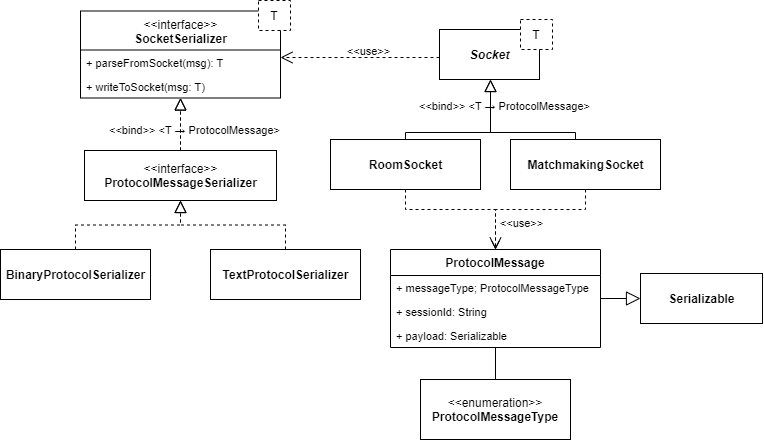
\includegraphics[scale=0.6]{images/4-design/communication_protocol.png}
	\caption{Websocket class diagram}
	\label{fig:websocket_communication_design}
\end{figure}
Regarding websockets instead, the design is more structured. A class diagram describing the main classes is shown in figure \ref{fig:websocket_communication_design}.
The \texttt{Socket} abstract class provides the main functionalities for a socket communication and allows to define the configurations for the connection: heartbeat rate and idle timeout. It is generic in T where T represents the type of messages sent through that socket . Two concrete implementations are provided for this class:
\begin{itemize}
	\item \texttt{RoomSocket}: used for the communication between client and rooms.
	\item \texttt{MatchmakingSocket}: used for the communication between client and matchmaking servicess
\end{itemize}
They both are Socket where the generic type T is a \texttt{ProtocolMessage}. This is indeed the class that defines the communication protocol between client and server. It has 3 fields to describe a message sent through a socket:
\begin{itemize}
	\item \textit{messageType} \\
	Used to identify the type of message that the client or the server want to send. The list of the possible message types is defined in the ProtocolMessageType enumeration.
	\item \textit{sessionId} \\
	This is used to identify the client that is sending the message through the socket. When a websocket connection is established between client and server, a unique id is genereated; the client must always uses the same sessionId to send messages through that socket.
	\item \textit{payload} \\ 
	An optional payload that can be carried with the massage. This is for example the field that is set when the developer use the 'sendMessage' method on the client room. It must be Serializable since it will eventually be serialized to be sent to the server.
\end{itemize}

In order for a Socket object to send and receive data, it must be able to serialize and deserialize the messages that pass through it. It uses for this purpose a \texttt{SocketSerializer} that has two methods: parsefromSocket and writeToSocket. This class is also generic in T that is the type of messages that needs to read and write.

Since \texttt{RoomSocket} and \texttt{MatchmakingSocket} needs to handle \texttt{ProtocolMessage}s we defined a \texttt{ProtocolMessageSerializer} interface that specifically defines a serializer for protocol messages. We implemented two types of serializers: \texttt{BinaryProtoclSerializer} and \texttt{TextProtocolSerializer}. The first one serialize protocol messages as binary data; the latter instead as text messages.
 
We have two different implementations because we initially thought to use json also for socket communication and this would be done by the \texttt{TextProtocolSerializer}. However we eventually decided to use binary representation both to improve performance and usability, so we switched to the \texttt{BinaryProtoclSerializer}


An example of a full interaction between client and server is shown in the sequence diagram in figure \ref{fig:create_room_seq}
\begin{figure}[]
	\hspace*{-1in}
	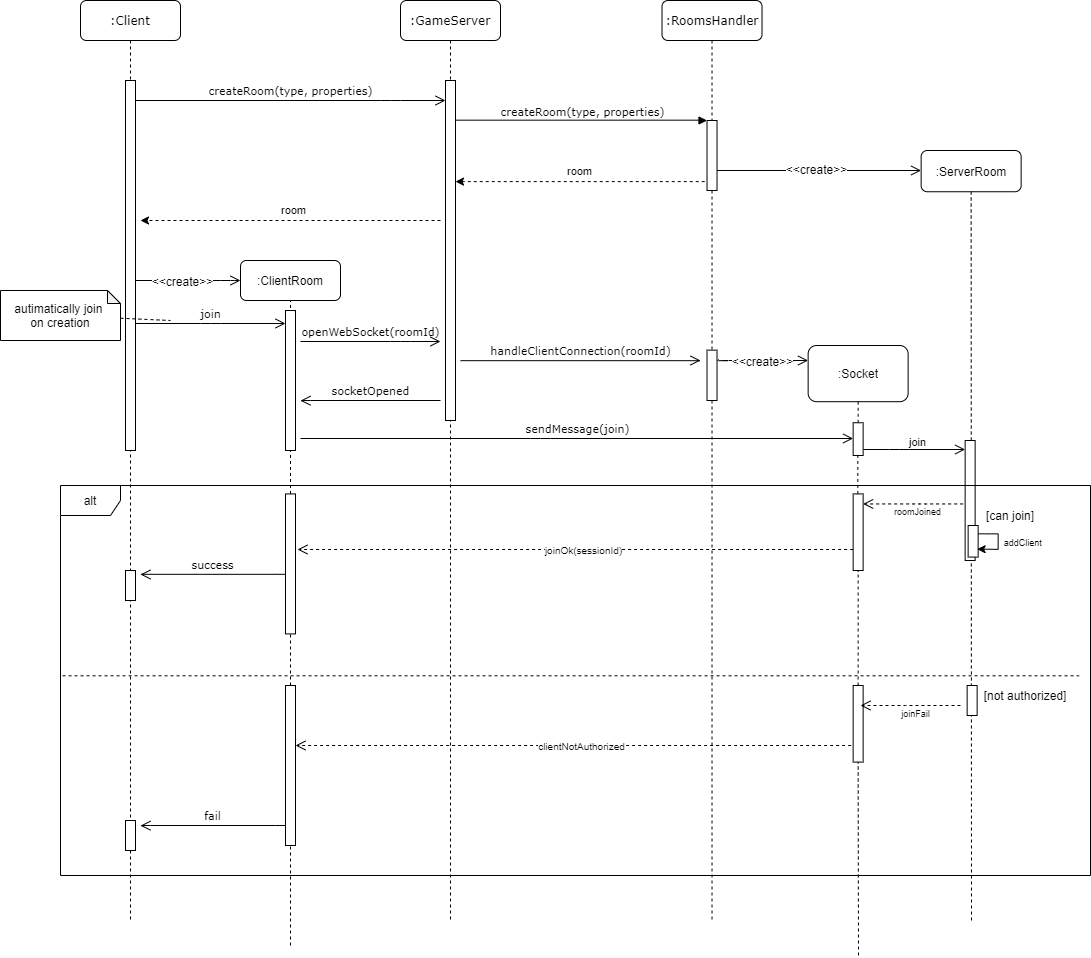
\includegraphics[scale=0.5]{images/4-design/crate_room_seq.png}
	\caption{Example of a client-server interaction upon a 'create room' request}
	\label{fig:create_room_seq}
\end{figure}